In this chapter, we validate our proposed solution with a set of meaningful queries over a real world dataset. To demonstrate the time efficiency of our approach, we select Neo4j community version 3.1.3 as the baseline. In the experiments, we test query processing time and space cost by running the queries using both our approach and Neo4j implementation.  The results show that our approach is about 20 times faster than the Neo4j implementation on average under the default settings (to be covered in Section \ref{Aspects of Interest}). Moreover, we assess and explain how each aspect in our system affects processing efficiency. Finally, we discuss our reflection on the Neo4j system.

%-------------------------------------------
---------------------------
\section{Experiment Setup}
%----------------------------------------------------------------------

%Our main focus is to evaluate different strategies for preprocessing and query evaluation. For instance, the threshold of “Is hot-structure” part in the diagram,  selection policy for materialized substructures in “Cube-Planner” and “Structure-Planner” , different heuristics when ranking sub-structures during decomposition in “Decomposition and Joining” etc.

There are two purposes of our experiments. First is to demonstrate the query processing efficiency of our proposed solution by comparing against the native Neo4j system. Second, we would like to test how different settings (of parameters and choices of strategies) in our solution affect query processing efficiency. %Experiments are run on a set of self-designed meaningful queries on a real-world dataset.

%----------------------------------------------------------------------
\subsection{Datasets}
%----------------------------------------------------------------------

We use the StackOverFlow dataset in our experiments that is generated by using raw information from https://archive.org/details/stackexchange. The dataset contains user-contributed content (such as user information, posts and etc.) on www.stackoverflow.com. The dataset contains 10 different node labels and 12 different edge labels.  Figure \ref{fig:metaexp} shows the meta graph of 8 node labels and 8 edge labels that are involved in our experiments. The data graph contains over 300 million vertices and more than 400 million edges and takes 44.5GB of storage.
\par

\begin{figure}[H]
	\centering
	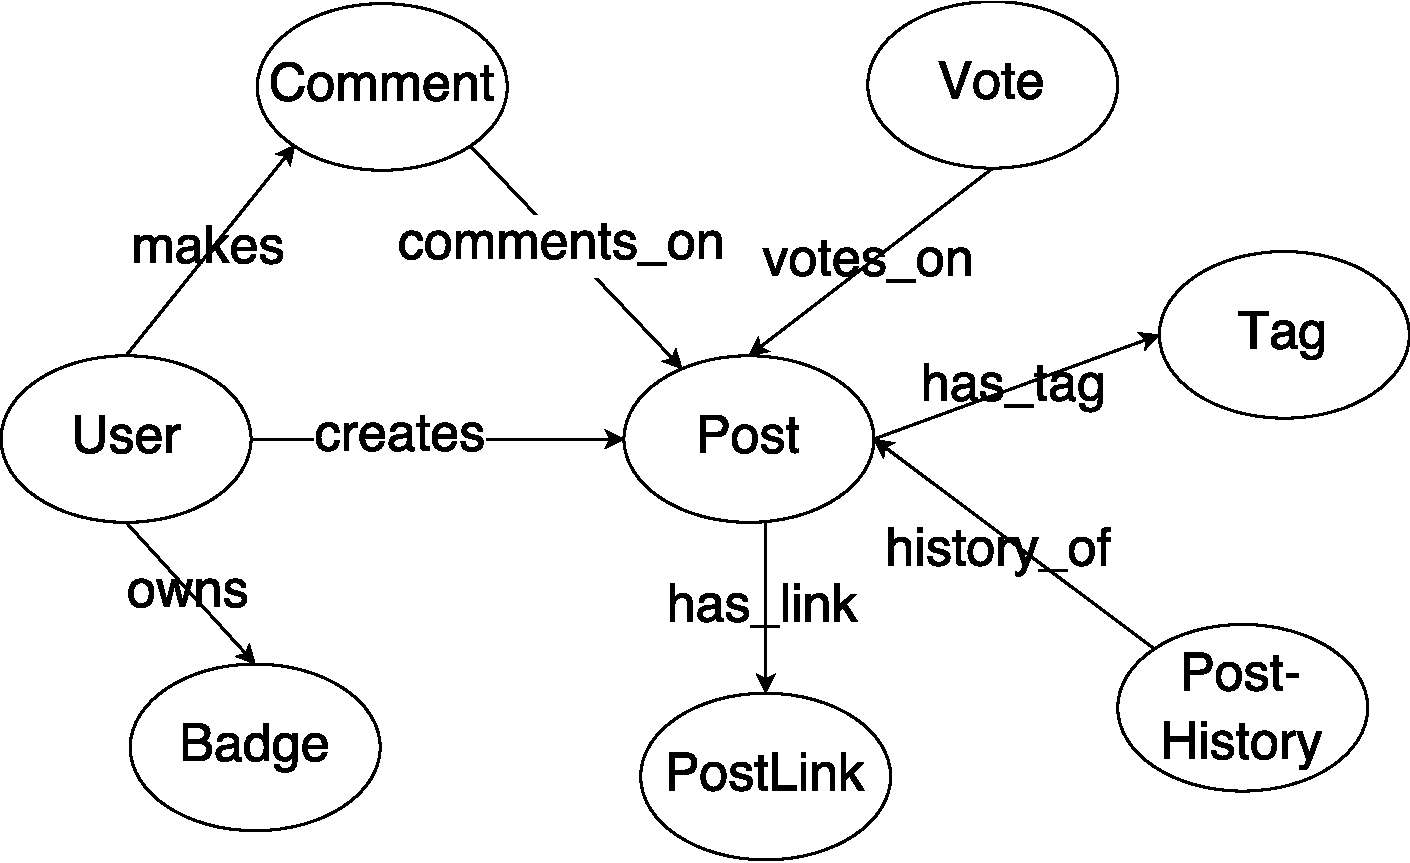
\includegraphics[scale=0.6]{pic/expmeta.pdf}
	\caption{The meta graph of StackOverFlow used in experiments.}
	\label{fig:metaexp}
\end{figure}

%\begin{figure}[H]
%	\centering
%	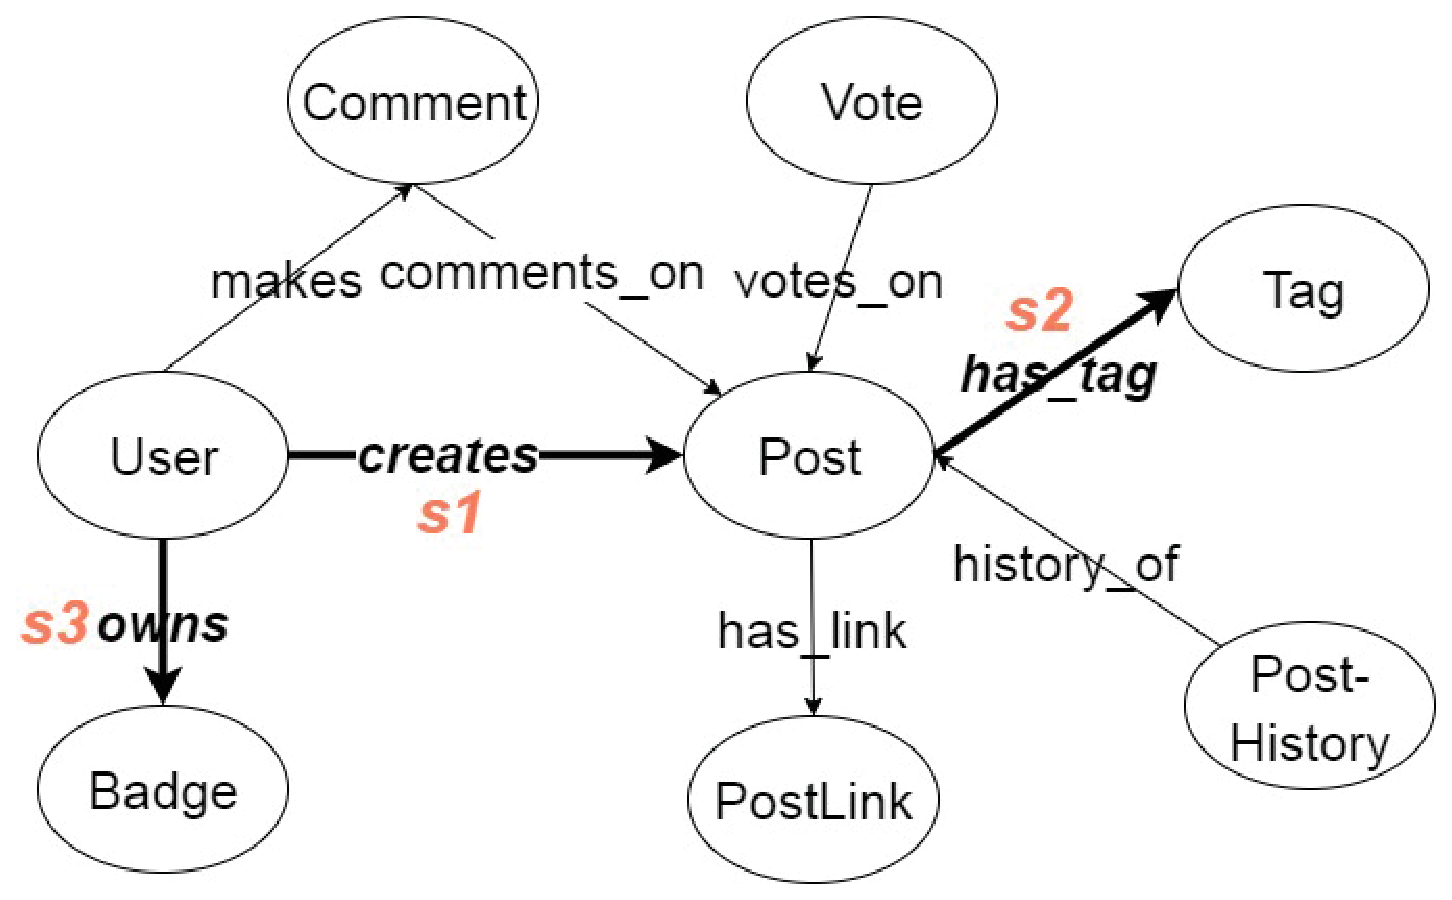
\includegraphics[scale=0.5]{pic/MetaExpS.eps}
%	\caption{The meta graph of StackOverFlow used in experiments.}
%	\label{fig:5:1}
%\end{figure}


%----------------------------------------------------------------------
\subsection{Query Workloads}
%----------------------------------------------------------------------
We design 24  queries against the StackOverFlow dataset given below. We randomly select 12 queries as the previous workload, leaving the rest 12 ones as the future workload.  %The meaning of each query is explained in the Appendix.


\textbf{Previous WorkLoad:}

P1 \hspace{3mm} User-Post: User.UpVotes, Post.Score=10

P2 \hspace{3mm} User-Post: User.UpVotes, (AVG)Post.Score

P3 \hspace{3mm} User-Post: User.Age, (SUM)Post.ActiveMonth

P4 \hspace{3mm} User-Post: User.CreationDate\_Year, Post.PostTypeId=1

P5 \hspace{3mm} Badge-User, User-Post, Post-Tag: Tag.TagName, User.CreationDate\_Year=2017

P6 \hspace{3mm} Badge-User, User-Post, Post-Tag: Tag.TagName, Badge.Name

P7 \hspace{3mm} Badge-User, User-Post:Badge.Date\_Year, (AVG)Post.Score

P8 \hspace{3mm} Badge-User, User-Post:Badge.Class, (AVG)Post.ActiveMonth

P9 \hspace{3mm} User-Post, Post-Tag: (AVG)User.Age, Tag.TagName

P10 \hspace{1.3mm} User-Post, Post-Tag: (AVG)User.UpVotes, Tag.TagName=Java

P11 \hspace{1.3mm} User-Post, Post-Vote: (AVG)User.UpVotes, Vote.VoteTypeId

P12 \hspace{1.3mm} Post-Comment, Post-PostLink: PostLink-LinkTypeId, (AVG)Comment-Score


\par
\textbf{Future WorkLoad:}

Q1 \hspace{3mm} User-Post: User.CreationDate\_Year=2017, Post.PostTypeId

Q2 \hspace{3mm} User-Post: (AVG)User.UpVotes,Post.Score

Q3 \hspace{3mm} User-Post: Post.ActiveMonth, (AVG)User.Age

Q4 \hspace{3mm} User-Post: User.CreationDate\_Year

Q5 \hspace{3mm} Badge-User, User-Post, Post-Tag: Tag.TagName, Badge.Class

Q6 \hspace{3mm} Badge-User, User-Post, Post-Tag: Tag.TagName, Badge.Date\_Year

Q7 \hspace{3mm} Badge-User, User-Post:Badge.Name, Post.PostTypeId

Q8 \hspace{3mm} User-Post, Post-Tag: User.UpVotes, Tag.TagName, Post.PostTypeId=2

Q9 \hspace{3mm} User-Post, Post-Tag:User.CreationDate\_Year, Tag.TagName

Q10 \hspace{1.3mm} Badge-User, User-Comment: Badge-Class, (AVG)Comment-Score

Q11 \hspace{1.3mm} Badge-User, User-Comment: Badge-Name, (AVG)Comment-Score

Q12 \hspace{1.3mm} Post-PostHistory, Post-Tag: Tag-TagName, PostHistory-PostHistoryTypeId





%----------------------------------------------------------------------
\subsection{System Setting}
%----------------------------------------------------------------------

We run the experiments on a Linux server with 256GB main memory. Our system is implemented in Java. We set the initial JVM memory to 100GB, and the maximal JVM memory to 200GB.

Our solution is developed on top of Neo4j Community v3.1.3. In the experiment, we set Neo4j's initial memory as 60GB and 200GB for the maximum usage. We use Neo4j's official Java driver (https://neo4j.com/developer/java/\#neo4j-java-driver) to interact with Neo4j server.

%----------------------------------------------------------------------
\section{Aspects of Interest}
\label{Aspects of Interest}
%----------------------------------------------------------------------

As we mentioned, there are two purposes of our experiments. In addition to the efficiency test, we would like to study how different settings in our system could affect query processing efficiency. We list the following aspects of interests to be tested. Default setting for each aspect is also presented. 

\textbf{Materialization}
\begin{itemize}
	
	\item  Space cost limit ($\sigma$ in Algorithm \ref{alg:5} in Section \ref{Structure Planner}) is set to 6GB by default. Results and discussion are presented in Section \ref{Space Cost Limit}.
	
	\item  Algorithms in materialized view selection described in Section \ref{Materialization Part}. For cuboid selection, we compare CubePlanner (in Section \ref{sec:CubePlanner}) with the ``Partial Materialization'' algorithm (PMA) proposed in Graph Cube \cite{DBLP:conf/sigmod/ZhaoLXH11}. For substructure selection we will compare StructurePlanner (in Section \ref{Structure Planner}) with the well-known maximal frequent pattern mining algorithm (FPM) \cite{DBLP:conf/dmkdttt/DewsnipM01}. In other tests, CubePlanner and StructurePlanner are used by default. Results are discussed in Sections \ref{CubePlannerPMA} and \ref{StructurePlanner vs FPM}, respectively.
	
	\item Frequency threshold for identification of “hot structures” ($\omega$ in Algorithm \ref{alg:1}). We set the default value to be 4; the intuition of default value, together with results and discussion are elaborated in Section \ref{Frequency Threshold}.
	
	\item Storage level for materialized views. We  compare main memory storage vs hard disk storage. Note that memory based materialization is set as the default in all other tests. Detailed discussion is provided in Section \ref{Storage Level for Merialized Views}.
	
\end{itemize}

\textbf{Future Query Processing}
\begin{itemize}
	\item  Choice of score functions in ranking substructures during the  ``Substructure Selection'' ($h(s)$ in Algorithm \ref{alg:SelectSubstrucre} discussed in Section \ref{Substructure Selection}). By default, $h(s)$ returns the score of $s$ calculated in StructurePlanner (as result of line 11 in Algorithm \ref{alg:5}). Results and explanations can be found in Section \ref{exp:Substructure Selection}.
	
	\item  Choice among using $Decompose\_Join$, $Decompose\_Join^{*}$ and $Decompose\_Join^{+}$ in ``Decomposition and Join'' in Section \ref{Query Decomposition}. We use $Decompose\_Join$ as the default method. Detailed discussion is in Section \ref{exp:DecomposeJoin}.
	
\end{itemize}

%Besides, we also ran experiments on the smaller dataset to see how performance varies in datasets of different sizes.

%----------------------------------------------------------------------
\section{Results and Discussion}
\label{Results and Discussion}
%----------------------------------------------------------------------
Following the interests of study listed above, we now present our experimental results.

%----------------------------------------------------------------------
\subsection{Our System vs. Neo4j}
\label{Our System vs. Neo4j}
%----------------------------------------------------------------------
We first show the time efficiency of our solution running in default settings against the native Neo4j implementation for the future workload.


\begin{figure}[H]
	\centering
	\includegraphics[scale=0.5, angle=270]{plot/neo4j.eps}
	\caption{Time efficiency on the future workload: our solution vs Neo4j.}
	\label{fig:neo4j}
\end{figure}

Figure \ref{fig:neo4j} shows the processing time for 12 future queries by both our system and Neo4j. It is worth pointing out that with an extra 5.7GB space cost for materialized views, our solution achieves remarkable efficiency improvement. Given the size of our dataset, this extra space is acceptable.

\begin{figure}[H]
	\centering
	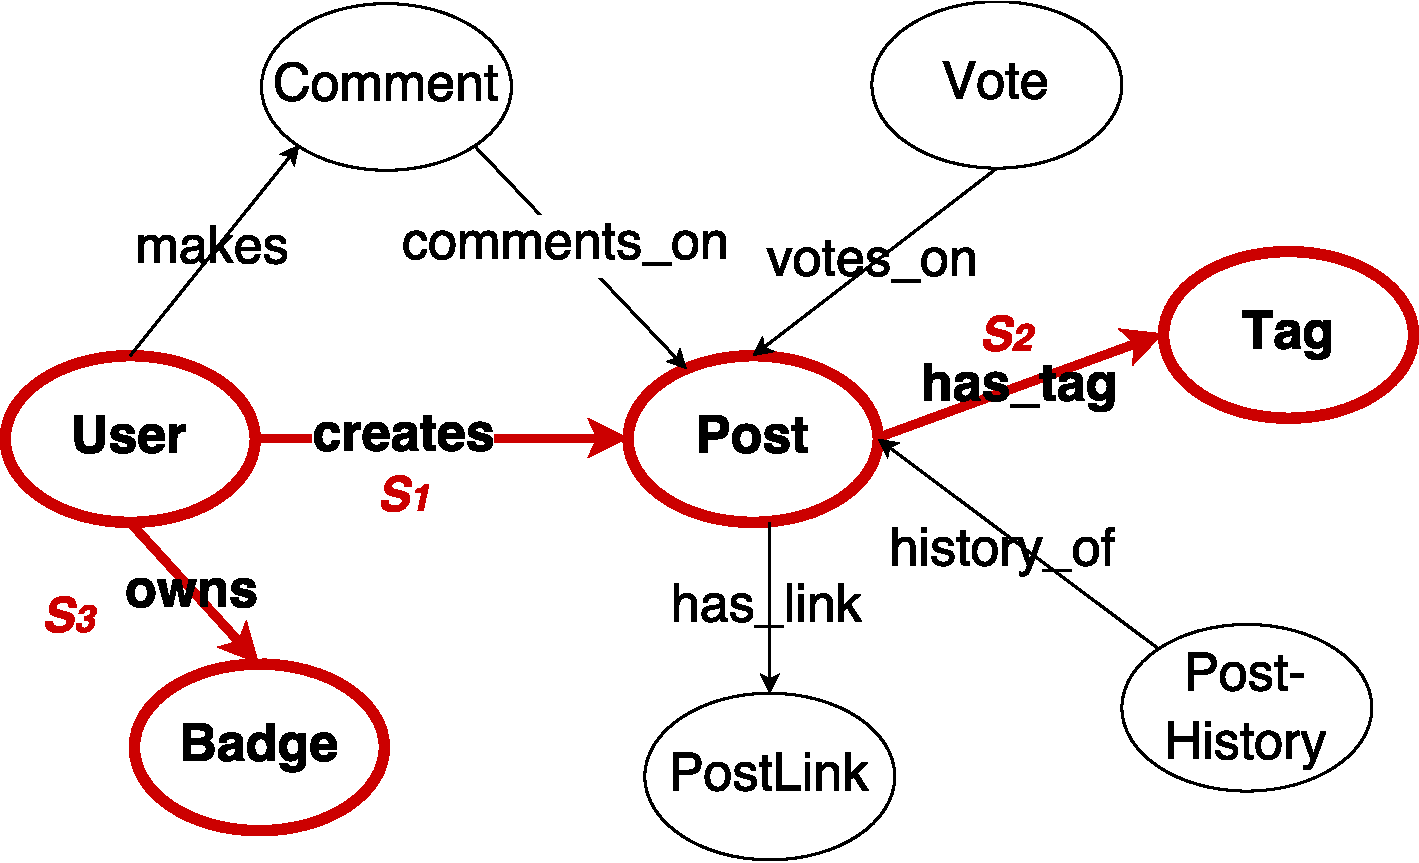
\includegraphics[scale=0.6]{pic/expmetaS.pdf}
	\caption{Substructure selected by StructurePlanner.}
	\label{fig:metagraphexperimenthot}
\end{figure}

We now detail how our system works over the 12 queries. First, \textit{User-Post} is identified as a ``hot structure'' as its frequency count is larger than or equal to the frequency count threshold. As a result, P1 - P4 are passed to the CubePlanner and P5 - P12 are passed to the StructurePlanner. Cuboids selected by CubePlanner are \{User.Age, Post.ActiveMonth\}, \{User.CreationDate\_Year, Post.PostTypeId\}, and \{User.UpVotes, Post.Score\}. Figure \ref{fig:metagraphexperimenthot} highlights substructures $S$ that StructurePlanner selects:  \textit{User-Post} ($s_1$), \textit{Post-Tag} ($s_2$) and \textit{Badge-User} ($s_3$). From the observation of the previous workload, we can tell that the StructurePlanner makes a good decision as these three substructures are able to cover most of previous queries.

We further explain the performance variance of the future workload. Overall improvement rate for Q1 - Q4 is more than 20000. This is because Q1 - Q4 are answered with a ``cuboid hit''. As a result, the time saving for these 4 queries are much greater than for Q5 - Q12 (which do not get a ``cuboid hit''). It worth pointing out that time complexities of cuboid aggregation and substructure joins are much different. The time complexity of a cuboid aggregation is bounded by the size of the Cartesian product of its dimensions. When it comes to substructure joins, however, the time complexity is related to the actual data sizes. Note that Q5 - Q9 are totally covered by $S$. In these cases, no ``complementary components'' are fetched from the Neo4j database.  Q10 - Q12 are partially covered by $S$.  Therefore, ``complementary components'' are fetched from the database, where a series of I/O operations increases the total time cost.  Overall, the improvement rate for Q5 - Q9 is around 28 times, while improvement rate for Q10 - Q12 ranges around 15 times. Clearly, our system could greatly improve query processing efficiency with an acceptable incremental space cost. While the improvement ratio varies in different scenarios of cuboid and structure ``hits''.




%----------------------------------------------------------------------
\subsection{Frequency Threshold}
\label{Frequency Threshold}
%----------------------------------------------------------------------
Frequency threshold $\omega$ can significantly affect the query processing efficiency. A change of $\omega$ may result in different ``hot structures'', followed by varied inputs for the CubePlanner and the StructurePlanner. It would further lead to different materialized view selection and overall query processing performance. As indicated in Section \ref{Overview of Materialization Part}, $\omega$ serves as a minimum threshold for building a cuboid over a ``hot structures'' (``cuboid hit'' assured). We think 4 is an appropriate choice for $\omega$ in our test case considering the frequency count of structures in previous workload (as shown in the table below).

\begin{center}
	\begin{tabular}{ | c | c |}
		\hline
		Structure	&Frequency	\\ \hline
		\textbf{User-Post} 	&\textbf{4} \\ \hline
		Badge-User, User-Post, Post-Tag 	&2 \\ \hline
		Badge-User, User-Post	&2 \\ \hline
		User-Post, Post-Vote	&2 \\ \hline
		User-Post, Post-Vote	&1 \\ \hline
		Post-Comment, Post-PostLink	&1 \\ \hline
	\end{tabular}
	\end {center}
	
	Suppose we lower $\omega$ to 2. \textit{Badge-User, User-Post, Post-Tag} will be ``hot structure''. As a result, cuboid selection over \textit{Badge-User, User-Post, Post-Tag} will be considered based on merely two queries (P5 and P6). Notice that Q5 and Q6, which have structure \textit{Badge-User, User-Post, Post-Tag}, will never get ``cuboid hit''. This is because properties Badge-Class in Q5 and Badge-Date\_Year in Q6 do not even appear in P5 and P6. That is to say, in this case any cuboid selected over \textit{Badge-User, User-Post, Post-Tag} will be useless. In addition, when $\omega$ is set to 2, input for StructurePlanner will be only two queries (Q11 and Q12). Note that structure frequency counts of these two queries are both 1. In other words, these are the most ``random'' queries. Note that the idea of StructurePlanner is to discover of useful substructures based on a sufficient number of ``less hot'' queries. In this case, two ``random'' queries are not the ideal input for the StructurePlanner.
	
	Suppose we increase $\omega$ to 5; then there will be no cuboid that is materialized in our test case. As a result Q1 - Q4 will be processed using substructure materialization ($s_1$). Although it is still faster than the native Neo4j system, the outstanding improvement ratio of ``cuboid hit'' cannot be achieved.
	
	Figure \ref{fig:omega} presents the total processing time under different settings of $\omega$. Note that no structure has frequency count of 3, therefore setting $\omega$ as 3 and 4 would categorize the same set of ``hot structures’’ and thus yield the same materialized views. We reach the conclusion that $\omega$ does have a significant effect over the system performance. Actually, determination on the value of $\omega$ is an interesting classification problem (based on the frequency count), which is left as future work since it is not the main focus of this thesis.
	
	\begin{figure}[H]
		\centering
		\includegraphics[scale=0.5, angle=270]{plot/omega.eps}
		\caption{Total processing time under different settings of $\omega$.}
		\label{fig:omega}
	\end{figure}
	
	
	%----------------------------------------------------------------------
	\subsection{Space Cost Limit}
	\label{Space Cost Limit}
	%----------------------------------------------------------------------
	As pointed out in Section \ref{Our System vs. Neo4j}, the space cost of our materialized views is 5.7GB, while the default space cost, $\sigma$, is set to 6GB. In this section, we study the effect of $\sigma$ on the query processing efficiency.  Figure \ref{fig:limit} shows how the total processing time varies with different space costs (which were caused by setting $\sigma$ to 6GB, 4GB, and 2.5GB, respectively). Apparently,  with more views being materialized, the total processing time decreases. However, the marginal benefit from materializing more views also decreases. This indicates that our Greedy Selection Framework (in Section \ref{s:Greedy Selection Framework}) successfully picks the proper candidates according to marginal benefits they would bring.
	
	\begin{figure}[H]
		\centering
		\includegraphics[scale=0.5, angle=270]{plot/limit.eps}
		\caption{Efficiency vs Space Cost}
		\label{fig:limit}
	\end{figure}
	
	%----------------------------------------------------------------------
	\subsection{Storage Level for Materialized Views}
	\label{Storage Level for Merialized Views}
	%----------------------------------------------------------------------
	As listed in Section \ref{Aspects of Interest}, by default, materialized views are stored as objects in main memory. This guarantees fast data access on the cost of extra memory consumption. Alternatively, materialized views can be serialized and stored as files on hard disks. Figure \ref{fig:disk} shows a comparison of the total query processing time using memory-based views and disk-based views. As expected,hard disk storage does not perform as fast as main memory storage. However, it is worth noting that  the drop in efficiency is acceptable. Such a drop in efficiency is due to the I/0 overhead in loading materialized views from disk files.
	
	One interesting question is what is the point of storing materialized views in files, since eventually they are to be read into the main memory. Our answer is that in cases when main memory is far too small for holding all selected views, materialization on disk provides an alternative.
	
	\begin{figure}[H]
		\centering
		\includegraphics[scale=0.5, angle=270]{plot/disk.eps}
		\label{fig:disk}
		\caption{Main memory storage vs hard disk storage}
	\end{figure}
	
	%----------------------------------------------------------------------
	\subsection{CubePlanner vs PMA}
	\label{CubePlannerPMA}
	%----------------------------------------------------------------------
	We compare CubePlanner in Section \ref{CubePlanner} in our solution with PMA in Graph Cube \cite{DBLP:conf/sigmod/ZhaoLXH11}. Figures \ref{fig:qjiawei} and \ref{fig:jiaweispace} show that CubePlanner outperforms PMA in both query processing efficiency and space cost. Cuboids selected by CubePlanner are $\{$User.Age, Post.ActiveMonth$\}$, $\{$ User.CreationDate\_Year, Post.PostTypeId$\}$, and $\{$User.UpVotes, Post.Score$\}$. While PMA selected $\{$User.Age, User.UpVotes, User.CreationDate\_Year, Post.PostTypeId, Post.Score, Post.ActiveMonth$\}$, $\{$User.Age, User.UpVotes, User.CreationDate\_Year, Post.PostTypeId, Post.ActiveMonth$\}$, $\{$User.Age, User.UpVotes, User.CreationDate\_Year, Post.PostTypeId, Post.Score$\}$.


\begin{figure}[H]
	\centering
	\includegraphics[scale=0.43, angle=270]{plot/qjiawei.eps}
	\caption{Time: CubePlanner vs PMA}
	\label{fig:qjiawei}
\end{figure}

\begin{figure}[H]
	\centering
	\includegraphics[scale=0.43, angle=270]{plot/jiaweispace.eps}
	\caption{Total cuboid space cost: CubePlanner vs PMA}
	\label{fig:jiaweispace}
\end{figure}

Both two approaches are considered as implementations of the Greedy Selection Framework given in Section \ref{s:Greedy Selection Framework}. The differences between the two implementations. CubePlanner uses the ratio of marginal benefit over space cost as a score for candidate ranking (line 11 in Algorithm \ref{alg:SingleCubePlanner}). While PMA only considers marginal benefit. That is to say, space cost is not taken into account in PMA. Moreover, PMA treats each combination of properties with an equal weight, regardless of how many times a combination has appeared in previous queries. For example, in our test case, the combination of {User.UpVotes, Post.Score} appears twice in previous workload. But PMA would treat {User.UpVotes, Post.Score} with the same weight as those combinations are not even queried in previous workload (\{User.UpVotes, Post.PostTypeId\} etc). As a result, CubePlanner adopts more information from previous workload and thus makes a better selection.

%----------------------------------------------------------------------
\subsection{StructurePlanner vs FPM}
\label{StructurePlanner vs FPM}
%----------------------------------------------------------------------
We compare our Algorithm \ref{alg:5} in StructurePlanner with FPM. In FPM we set the minimum support to 2 considering the frequency count as listed in the table in Section \ref{Frequency Threshold}. These two ways provide different substructure selections which lead to different processing efficiency. Figures \ref{fig:fpmtotal} and \ref{fig:fpmspace} show that our StructurePlanner outperforms FPM in both efficiency and space cost.

\begin{figure}[H]
	\centering
	\includegraphics[scale=0.43, angle=270]{plot/fpm.eps}
	\caption{Total processing time for future workload: StructurePlanner vs FPM}
	\label{fig:fpmtotal}
\end{figure}

\begin{figure}[H]
	\centering
	\includegraphics[scale=0.43, angle=270]{plot/fpm_space.eps}
	\caption{Space cost: StructurePlanner vs FPM}
	\label{fig:fpmspace}
\end{figure}

Figure \ref{fig:metagraphexperimenthot} highlights three selected substructures by StructurePlanner. As mentioned, it is a good selection as these three substructures are able to cover most of the previous queries. However, FPM selects \textit{Badge-User, User-Post, Post-Tag}, which is a bad selection because it is useful only for Q5 and Q6. In addition, materialization of \textit{Badge-User, User-Post, Post-Tag} results in even more space cost than materialization of the three edges separately (as selected by StructurePlanner). Figure \ref{fig:qfpm} details processing time for each query. FPM only outperforms StructurePlanner on Q5 and Q6. This is because Q5 and Q6 would be able to perform aggregation over the materialization of \textit{Badge-User, User-Post, Post-Tag} when FPM is applied. While table joins of $s_1$, $s_2$ and $s_3$ are required if StructurePlanner is applied, which clearly is more time consuming. However for Q7 - Q12, StructurePlanner is the winner as it gets at least a partial ``substructure cover'', while the FPM-selected structure is not helpful at all.

\begin{figure}[H]
	\centering
	\includegraphics[scale=0.5, angle=270]{plot/qfpm.eps}
	\caption{Processing time for each query: StructurePlanner vs FPM}
	\label{fig:qfpm}
\end{figure}


%----------------------------------------------------------------------
\subsection{Substructure Selection}
\label{exp:Substructure Selection}
%----------------------------------------------------------------------

In our experiment, $h(s)$ in Algorithm \ref{alg:SelectSubstrucre} does not make any difference during ``Substructure Selection''. This is because the three selected substructures do not share any edges. Note that scenarios in Section \ref{Substructure Selection} where multiple valid combinations of materialized substructures exist only happen when materialized substructures have overlaps.

%----------------------------------------------------------------------
\subsection{Decompose\_Join}
\label{exp:DecomposeJoin}
%----------------------------------------------------------------------
We now present the experiments comparing  $Decompose\_Join$, $Decompose\_Join^{*}$ and $Decompose\_Join^{+}$ in ``Decomposition and Join'' (presented in Section \ref{Query Decomposition}). Three different implementations in ``Decomposition and Join'' would lead to different processing performance for Q10 - Q12, as they are partially covered by $S$ and fetching ``complementary components'' from Neo4j is necessary. Figure \ref{fig:threeall} provides the processing time for Q10 - Q12 using the three approaches. $Decompose\_Join^{*}$ performs  better than $Decompose\_Join$ in Q10. This is because $Decompose\_Join^{*}$ passes to Neo4j candidate IDs of users who have badges, which provides a considerable ``filtering effect'' when fetching \textit{User-Comment}. As a result, $Decompose\_Join^{*}$'s processing time for fetching \textit{User-Comment} is reduced. Besides, its time for joining \textit{Badge-User} and \textit{User-Comment} also decreases because the table size of \textit{User-Comment} is smaller than that of $Decompose\_Join$, thanks to the ``filtering effect''. This is reflected in Figure \ref{fig:threejoin}, where the time for join is saved in $Decompose\_Join^{*}$. However $Decompose\_Join^{*}$ performs badly for Q12. This is because the ``filtering effect'' of \textit{Post-Tag} in fetching \textit{Post-PostHistory} is small as most posts have tags. In addition, $Decompose\_Join^{*}$ has an overhead of scanning the \textit{Post-Tag} table in order to get the set of candidate IDs. It explains why $Decompose\_Join^{*}$ takes longer time in processing Q12. Figure \ref{fig:threetotal} gives the total processing time for Q10 - Q12 using the three approaches. We see that $Decompose\_Join^{+}$ has best overall performance. To explain,  $Decompose\_Join^{+}$ is able to choose the faster approach when fetching ``complementary components'' from Neo4j in scenarios like Q10 and Q12 with  the cost of a cheap trial query (as discussed in Section \ref{Query Decomposition}). Note that the time cost for a ``trial query'' is bounded by a constant sample size, and is not proportional to actual data size in the dataset. Figure \ref{fig:threesample} shows that the time cost ``trial query'' is negligible compared to the overall processing time.


\begin{figure}[H]
	\centering
	\includegraphics[scale=0.43, angle=270]{plot/threeall.eps}
	\caption{Processing time for Q10 - Q12 by three approaches.}
	\label{fig:threeall}
\end{figure}


\begin{figure}[H]
	\centering
	\includegraphics[scale=0.43, angle=270]{plot/threejoin.eps}
	\caption{Joining time in processing Q10 - Q12 by three approaches.}
	\label{fig:threejoin}
\end{figure}
\begin{figure}[H]
	\centering
	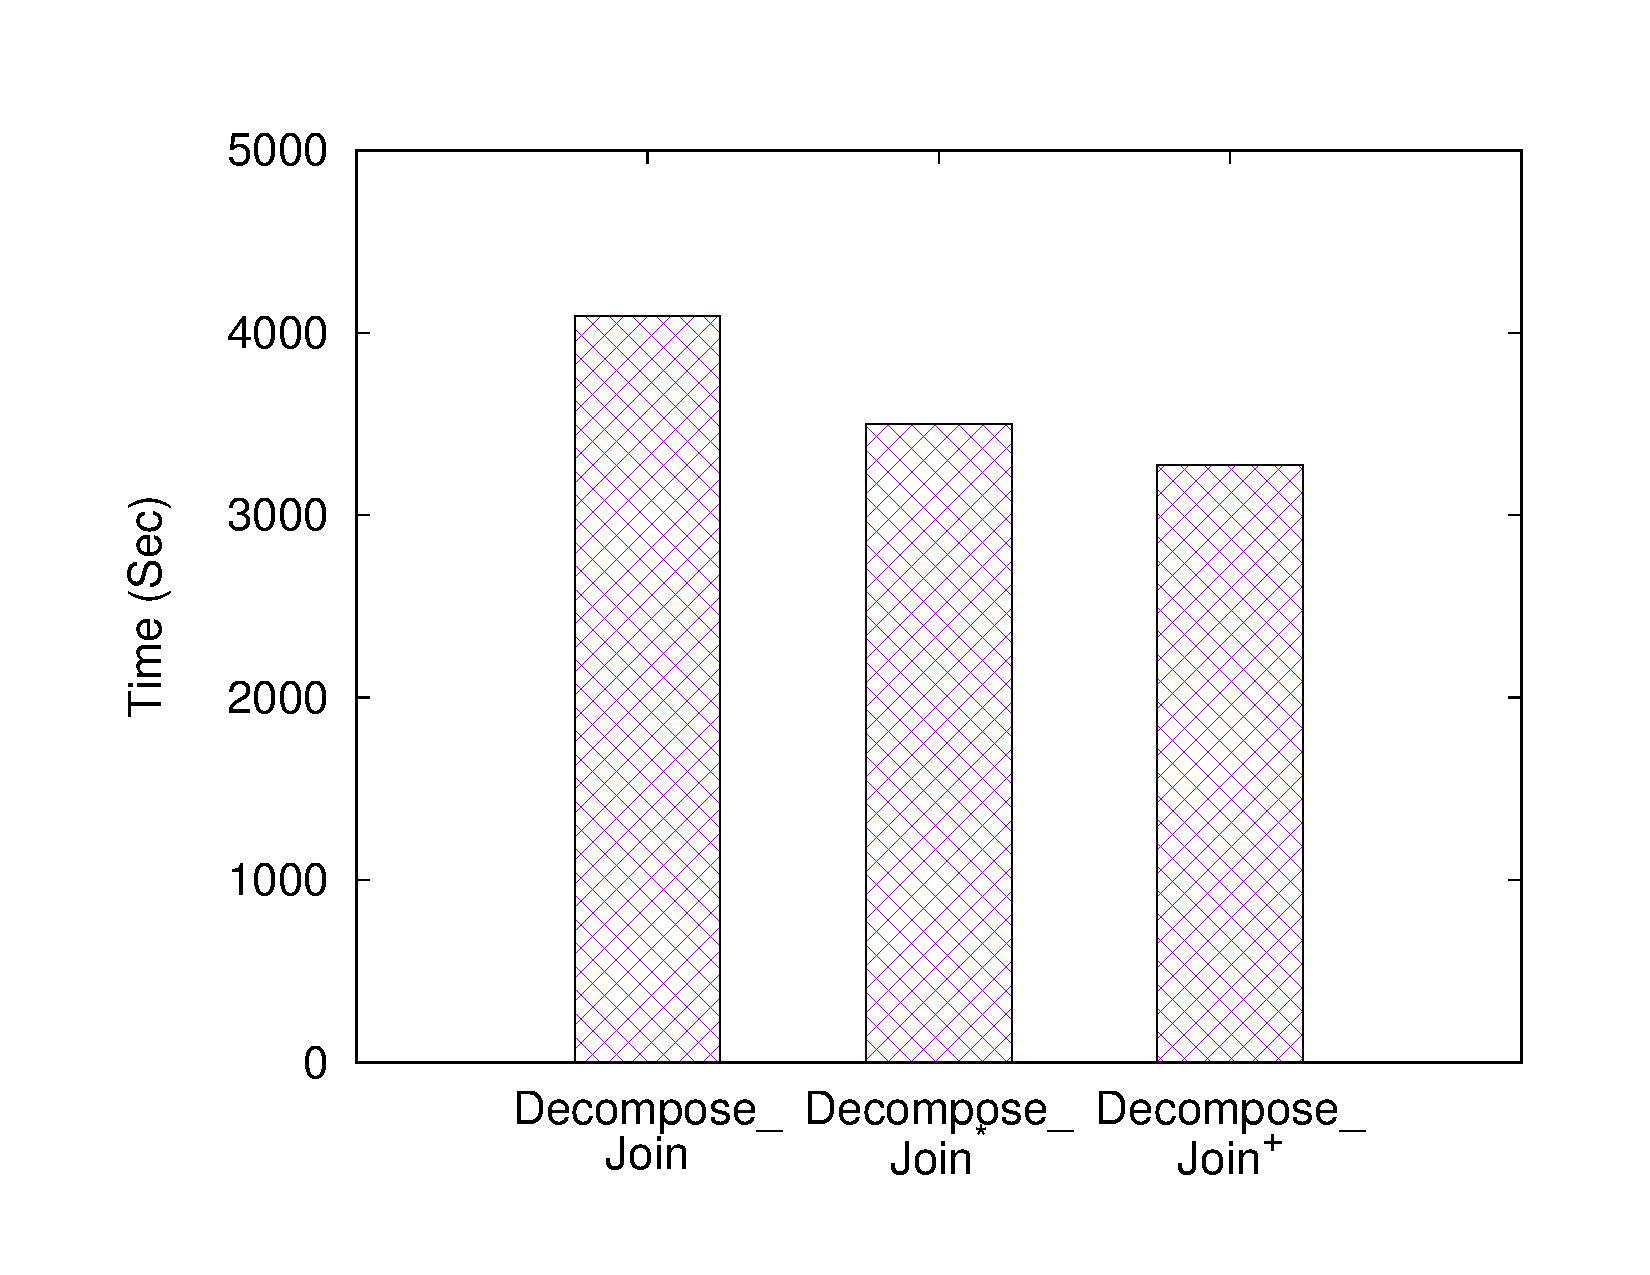
\includegraphics[scale=0.42]{plot/threetotal.pdf}
	\caption{Total processing time for Q10 - Q12 by three approaches.}
	\label{fig:threetotal}
\end{figure}

\begin{figure}[H]
	\centering
	\includegraphics[scale=0.42, angle=270]{plot/threesample.eps}
	\caption{Total processing time vs ``trial query'' processing time.}
	\label{fig:threesample}
\end{figure}

To conclude, ``filtering effect'' is an important factor in the performance of these three different implementations of ``Decomposition and Join''. In general, $Decompose\_Join^{+}$ is the recommended approach as it is able to select the better solution with a small cost of ``trial query''.


%%----------------------------------------------------------------------
%\subsection{Large DataSet vs Small DataSet (Only graphs not ready)}
%%----------------------------------------------------------------------
%Besides StackOverFlow dataset (45.8GB), we also tested on a smaller ``StackExchange-Math'' dataset of size 2.57GB. Like StackOverFlow dataset, StackExchange-Math dataset is about a mathematics Q\&A forum (https://math.stackexchange.com).  The raw data of StackExchange-Math dataset also comes from https://archive.org/details/stackexchange and it has exactly the same schema as StackOverFlow dataset.
%
%Figure \ref{} compares efficiency improvement rate for large dataset and smaller dataset. We see that our system achieved even better performance on larger dataset.

%----------------------------------------------------------------------
\subsection{Reflections on Neo4j}
%----------------------------------------------------------------------
During the experiments, we found that Neo4j uses a na\"ive approach to result size estimation for aggregation queries. It simply takes the square root of table length before aggregation as the estimated size for the aggregated result, regardless of which properties are being aggregated. Such a method leads to a huge bias in the estimation.

For example, Figure \ref{fig:wrong1} presents Neo4j's execution plans for queries \textit{User-Post: User.Age} and \textit{User-Post: ID(User), ID(Post)}, respectively. Obviously the latter query should have much larger estimated result size than the former one. However Neo4j returns exactly the same estimated result size by simply taking the square root of table length (216791 estimated rows in ``Projection'' step) in the previous step.

%explain match (u:User)-[]-(p:Post) return u.Age, count(*)

\begin{figure}[H]
	\centering
	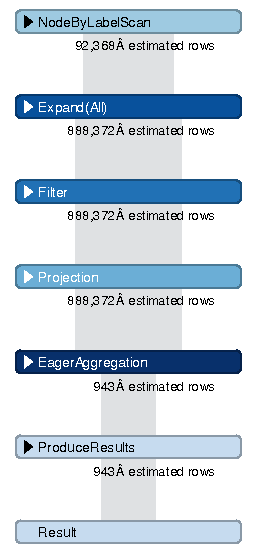
\includegraphics[scale=1.5]{pic/wrong.pdf}
	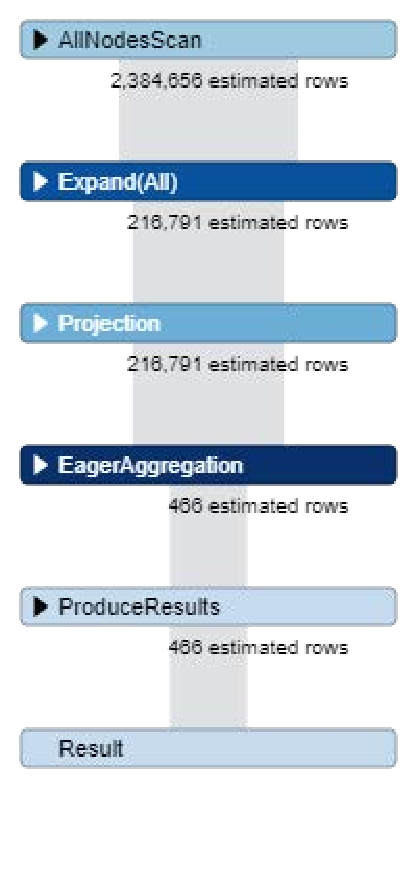
\includegraphics[scale=1.5]{pic/wrong2.pdf}
	\caption{Execution plans for \textit{User-Post: User.Age} and \textit{User-Post: ID(User), ID(Post)}.}
	\label{fig:wrong1}
\end{figure}

This is why we use the Cartesian product of dimensions to estimate cuboid sizes in ``Single CubePlanner''(covered in Section \ref{sec:CubePlanner}).
